\documentclass[a4paper]{article}
\usepackage{listings}
\usepackage{qtree}
\usepackage{xcolor}
\usepackage{forest}
\usepackage{multicol}
\setlength{\columnsep}{3cm}
\usepackage{parskip}
\usepackage{changepage}
\usepackage[T1]{fontenc}
\usepackage{amsmath}
\usepackage{hyperref}
\usepackage{listings}
\usepackage{amsthm}
\usepackage{amssymb}
\usepackage{float}
\usepackage[utf8]{inputenc}
\usepackage{graphicx}
\usepackage[italian]{babel}
\usepackage{thmtools}
\newtheorem*{theorem}{Teorema}
\newtheorem*{definition}{Definizione}
\newtheorem{example}{Example}
\newenvironment{dimostrazione}{\textit{Dimostrazione}:\begin{adjustwidth}{1cm}{}}{\end{adjustwidth}}
\newcommand{\imp}[1]{\textbf{\textit{#1}}}

\begin{document}

\author{Lorenzo Dentis, lorenzo.dentis@edu.unito.it}
\title{Risposte AlgComp}
\maketitle

\section{Brute-force e certificazione}
\subsection{A.1}
Posto un array $V$ di $n$ elementi individuo due indici, $i$ e $j$.\\L'idea è di mantenere gli elementi $[0 ... j-1]$ fissi ed andare a generare tutte le permutazioni dei restanti elementi $[j ... n-1]$grazie all'indice $i$.

Ad ogni incremento dell'indice $i$ segue una sequenza di chiamate ricorsive che hanno lo scopo di effettuare uno swap fra l'elemto di indice $i$ e l'elemento di indice $j$ e poi incrementare $j$ scendendo nell'albero della ricorsione fino alla condizione $j=i$, quando $i$ viene di nuovo incrementato.Intuitivamente $j$ indica la profondità della ricorsione, $i$ indica l'ampiezza.
\begin{itemize}
	\item \textbf{Punto 1}:L'algoritmo è completo in quanto genera $n!$ permutazioni, ed è corretto in quanto sono tutte distinte.\\Le permutazioni generate sono esattamente $n!$ in quanto alla "radice" dell'albero avrò $n$ chiamate ricorsive (con $i = 0, i=1, ... i= n-2, i=n-1$ ).Invece al livello di profondità $j$ i primi $j$ elementi del vettore risulteranno fissi ed avrò solo $n-1-j$ chiamate ricorsive.\\Considerando che il valore di $j$ viene incrementato di una unità ad ogni "livello" di ricorsione fino all' $n-(n-1)$esimo livello ottengo questa semplice equazione: \begin{center}$calls = n * (n-1) * ...(j-1$volte$)... * 1$\end{center}Che non è altro che $n!$\\
		Le permutazioni sono tutte distinte perchè $i$ e $j$ non assumono mai due volte lo stesso valore, posto che ogni elemento del vettore sia distinto.Di conseguenza lo "swap" avverrà sempre tra due elementi differenti ad ogni chiamata ricorsiva, generando sottoalberi uno diverso dall'altro e di conseguenza sequenze differenti.
	\item \textbf{Punto 2}:Un algoritmo che generi \textit{tutti i sottoinsiemi di elementi} può essere realizzato organizzando lo spazio degli stati in sottoinsiemi.
		Al posto che intendere una permutazione come sequenza di elementi la si può vedere come una serie di \textit{scelte}, ovvero booleani.Essenzialmente si va a generare un vettore $B$ di booleani i cui elementi indicano se il corrispondente elemento di $V$ va considerato o meno.\\
		Se $B[i] == True$ allora $V[i]$ fa parte del sottoinsieme che si sta generando.\\
		In tal modo otteniamo il \textbf{PowerSet} di $V$, che è completo (cioè le permutazioni sono $2^n$) in quanto ogni cella del vettore $B$ può avere solamente valore binario e le celle sono $n$.
		E' invece corretto, di nuovo posto che gli elementi siano distinti, in quanto non vi è alcuno \textit{"swap"} e nessuna sequenza è ripetuta più volte. Ogni sequenza di \textit{True/False} varia dalla precedente di una scelta, garantendo sequenze distinte.
\end{itemize}
\begin{figure*}[!ht]
\centering
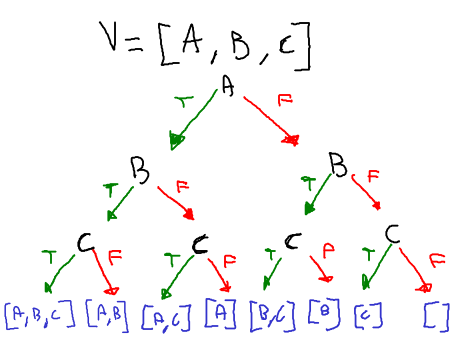
\includegraphics[scale = 0.5]{./img/A1_2.png}
\caption{PowerSet di [a,b,c]} \label{FIG:PowerSet}
\end{figure*}
\subsection{A.2}
Definizione formale di una permutazione (definizione ricorsiva):
\begin{figure*}[!ht]
\centering
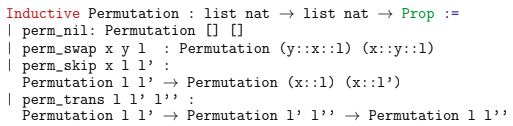
\includegraphics[width=0.7\textwidth]{./img/permutazione_ricorsiva.png}
\caption{Definizione ricorsiva di una permutazione} \label{FIG:recursive_permutation1}
\end{figure*}
\begin{itemize}
	\item perm\_nil: [ ] è permutazione di [ ] (lista vuota è permutazione di se stessa)
	\item perm\_swap: $\forall x,y \in Elements$ e $\forall l \in Lists$ $[y::x::l]$ e $[x::y::l]$ sono una permutazione dell'altra
	\item perm\_skip: dato $x \in Elements$, se $l \in Lists$ è permutazione di $l' \in Lists$ $\Rightarrow [x::l]$ è permutazione di $[x::l']$
	\item perm\_trans: date $l, l', l'' \in Lists$ se $l$ permutazione di $l'$ e $l'$ permutazione di $l'' \Rightarrow l$ è permutazione di $l''$ 
\end{itemize}
\begin{theorem}[Riflessività] $\forall l \in Lists$ Permutation $l$ $l$\end{theorem}
\textit{Dimostrazione}:
\begin{adjustwidth}{2cm}{}
	\textit{caso base}: $l$ = [ ], vale per definizione grazie a perm\_nil\\
	\textit{caso induttivo}: $l = [h::t]$ con $h \in Lists$ e $t \in ELements$.\\
	Grazie all'ipotesi induttiva si può affermare \textit{Permutation} $t$ $t$ e quindi per perm\_skip \textit{Permutation} $[h::t]$ $[h::t]$. Dato che $l = [h::t]$ abbiamo che \textit{Permutation} $l$ $l$.
\end{adjustwidth}
\begin{theorem}[Simmetria] $\forall l,l' \in Lists$, Permutation $l$ $l'$ $\Rightarrow $ Permutation $l' \; l$\end{theorem}
\begin{dimostrazione}
	Assumo che $l$ sia permutazione di $l'$, ma allora devo poter applicare la definizione di \textit{Permutazione}, i 4 casi di figura~\ref{FIG:recursive_permutation1} 


	\textit{primo caso}: $l=[] \; l'=[]$, la proprietà \emph{perm\_nil} ci garantisce sia che $P \;l \; l'$ che $P \; l'\; l$. $l'$ ed $l$ si sono "scambiate"


	\textit{secondo caso}: $l = x::y::t$, $l'= y::x::t$. Assunta vera $P \; l \, l'$, cioè $P \; x::y::t \; y::x::t$, grazie a \emph{perm\_swap} si può affermare $P \; y::x::t \; x::y::t$, cioè $P \; l' \; l$

	\textit{terzo caso}: caso induttivo, è stata applicata \textit{perm\_skip} all'ipotesi quindi $l = x::t$ e $l' = x::t'$ e per definizione $P \; t \, t'$.
	Ma per ipotesi induttiva $P \; t \, t' \Rightarrow P \; t' \, t'$, riapplicando \textit{perm\_skip} ottengo $P \; x::t' \; x::t$ che è esattamente $P \; l' \, l$

	\textit{quarto caso}: caso induttivo, è stata applicata \textit{perm\_trans} all'ipotesi e quindi deve esistere una lista intermedia $l''$ t.c. $P\; l\, l''$ e $P \; l''\, l'$ sono vere.
	Applicando l' ipotesi induttiva alle due affermazioni precedenti otteniamo:$P\; l''\, l$ e $P \; l'\, l''$.\\
	Applicando \textit{perm\_trans} ad entrambe si ottiene $P \; l' \, l$
\end{dimostrazione}
\subsection{A.3}
Dimostrare che è algoritmo che genera permutazioni di una lista di elementi è completo significa dimostrare che genera $n!$ permutazioni, con $n$ pari al numero di elementi. Formalmente:
\begin{theorem}[Completezza] $\forall l \in Lists$, $len($\textit{permutation} $l) = len(l)!$\end{theorem}
\begin{dimostrazione}
	\textit{caso base}: $l$ = [ ]\\
	In questo caso $len(l)! = 0! = 1$.\\
	Allo stesso modo $len(permutation)$ [ ] $= len($[ [ ] ]$) = 1$.\\
	Quindi $len($\textit{permutation} $l) = len(l)!$
	
	\textit{Caso induttivo}: $l = h::t$, quindi l'enunciato da dimostrare è\\ $len($\textit{permutation} $[h::t]) = len([h::t])!$\\
	$len(h::t) = 1 + len(t)$\\
	Quindi $len(distribute$ $a$ $[h::t]) = 2 + len(t)$ che per il Lemma distribute\_lenght diventa $len((a::t)::distribute$ $a$ $t) = 2 + len(t)$
	INSERIRE FOTO LEMMA DISTRIBUTE
	DA FARE
\end{dimostrazione}
\subsection{A.4}
\begin{itemize}
	\item \textbf{Permutazioni}:Si può individuare una \emph{risposta} al problema \textbf{Valutazione} generando l'albero di tutte le possibili permutazioni:
		\begin{center}	\scalebox{0.8}{\Tree [  [ [ .1 [  [ .2 [.3 4 ] [.4 3 ] ] [ .3 [.2 4 ] [ .4 2 ] ] [ .4 [ .2 3 ] [ .3 2 ] ] ] ] [ .2 [ [ .1 [ .3 4 ] [ .4 3 ] ] [ .3 [ .1 4 ] [ .4 1 ] ] [ .4 [ .1 3 ] [ .3 1 ] ] ] ] [ .3 [ [ .1 [ .2 4 ] [ .4 2 ] ] [ .2 [ .1 4 ] [ .4 1 ] ] [ .4 [ .1 2 ] [ .2 1 ] ] ] ] [ .4 [ [ .1 [ .3 2 ] [ .2 3 ] ] [ .3 [ .1 2 ] [ .2 1 ] ] [ .2 [ .1 3 ] [ .3 1 ] ] ] ] ] ]}
		\end{center}
		In questo albero un ramo individua una permutazione dell'insieme di partenza, di conseguenza basta percorrerlo calcolando di volta in volta il voto massimo finchè questi non supera il valore fissato (in questa istanza 9).Si ottiene quindi una soluzione, data dalla sequenza di "voti" ottenuta partendo dalla radice e percorrendo il ramo corrispondente fino al padre del nodo che causa il superamento del voto massimo.
		Eseguendo questa operazione su tutti i rami dell'albero si ottengono tutte le \emph{soluzioni}, scegliendo le soluzioni con votazione migliore si ottengono una o più \emph{risposte}.
	\item \textbf{Sottoinsiemi}:Si può individuare una \emph{risposta} al problema \textbf{Valutazione} generando l'albero di tutte le possibili scelte:
		\begin{center}
			\begin{forest}
				for tree={ l sep=20pt, s sep=20pt}
			[1 [2, edge label = {node[midway,left,green] {T}} [3, edge label = {node[midway,left,green] {T}}[4, edge label = {node[midway,left,green] {T}}] [4, edge label = {node[midway,right,red] {F}}]] [3, edge label = {node[midway,right,red] {F}}[4, edge label = {node[midway,left,green] {T}}] [4, edge label = {node[midway,right,red] {F}}]]][2, edge label = {node[midway,right,red] {F}} [3, edge label = {node[midway,left,green] {T}}[4, edge label = {node[midway,left,green] {T}}] [4, edge label = {node[midway,right,red] {F}}]] [3, edge label = {node[midway,right,red] {F}}[4, edge label = {node[midway,left,green] {T}}] [4, edge label = {node[midway,right,red] {F}}]]]] 			\end{forest}
		\end{center}
		A seconda che si scelga un ramo o l'altro la domanda sarà inclusa nella possibile \emph{soluzione} quindi percorrendo un ramo fino alla foglia si giunge sempre ad una sequenza di voti.
		Non tutti i sottoinsiemi così generati sono però \emph{soluzioni}, in quanto alcuni superano il vincolo del voto massimo ammesso (in questo caso 9); considerando solo le \emph{soluzioni} e scegliendo quelle aventi la migliore votazioni si ottengono una o più \emph{risposte}
\end{itemize}
\section{Backtrack}
\section{Branch\&Bound}
\subsection{C.1}
\label{SEC:C_1}
\begin{itemize}
	\item \textcolor{gray}{\textit{dead node}}: radice di sotto-alberi che non sono più espandibili, perchè completi o a causa del pruning
		\item \textcolor{red}{\textit{live node}}: nodo "vivo", cioè alcuni dei suoi figli sono ancora da espandere
		\item \textcolor{red}{\textit{E-node}}: L' \textit{expanded node} è il nodo che si sta visitando in questo momento, cioè il nodo del quale si sta per generare un figlio.L' \textit{E-node} e per definizione un \textit{live node}.
\end{itemize}
A seconda di come si gestisce la visita dei nodi e l'assegnamento dell' \textit{E-node} si può generare una visita dello spazio degli stati differente.
\begin{figure*}[!ht]
\centering
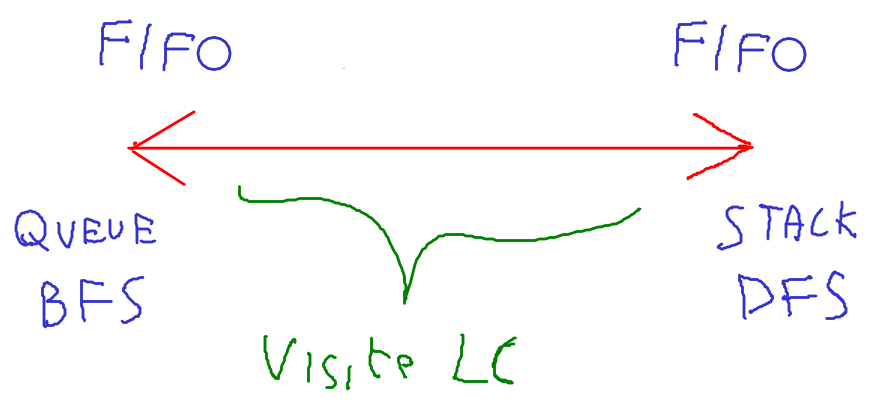
\includegraphics[width=0.7\textwidth]{./img/C_1.png}
\caption{criteri di scelta} \label{FIG:C_1}
\end{figure*}\\
Come mostrato in figura~\ref{FIG:C_1} FIFO e LIFO sono "i due estremi di un ventaglio di possibili criteri di scelta".
Gestendo i live node com uno \emph{stack} e quindi andando ad estrarre l'ultimo nodo inserito si ottiene una visita \textit{depth-first} in cui si trasferisce la condizione di essere \textit{E-node} dal padre al figlio appena generato.
In tal modo un nodo non diventa "\emph{dead} finchè tutti i suoi figli non sono stati visitati, di conseguenza si tende ad arrivare al fondo dell'albero degli stati il più in fretta possibile.
\begin{figure*}[!ht]
\centering
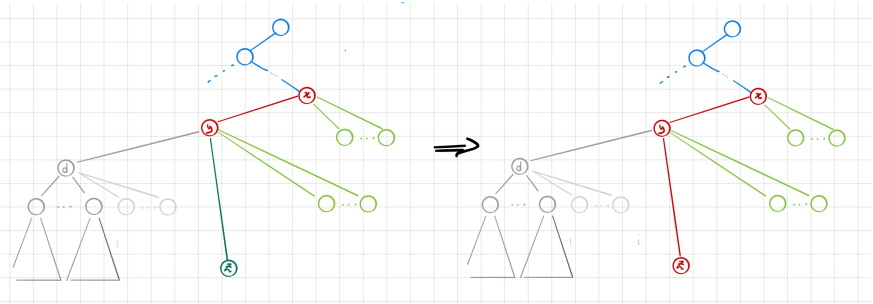
\includegraphics[width=1\textwidth]{./img/C_1_DFS.png}
\caption{visita in profondità} \label{FIG:C_1_DFS}
\end{figure*}\\
In maniera diametralmente opposta funziona la gestione dei nodi con una \emph{queue} in cui il primo nodo inserito è il primo ad essere estratto.Questa politica genera una visita \textit{breadth-first} in cui prima di passare ai nodi del livello successivo i nodi del livello attuale vengono tutti visitati, una volta generati tutti i figli di un nodo questi diventa "dead".
Ciò porta a visite dello spazio degli stati che prima di giungere alle foglie dell'albero degli stati "esplorano" tutte le possibilità.
\begin{figure*}[!ht]
\centering
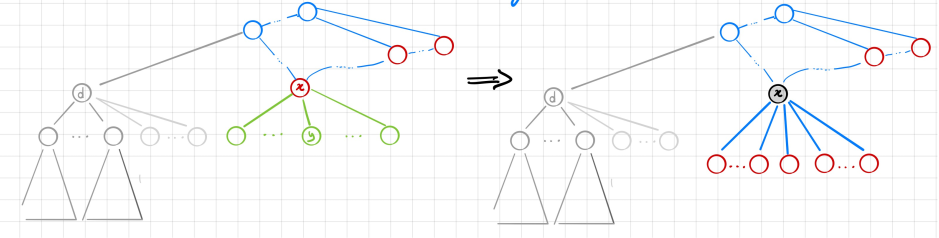
\includegraphics[width=1\textwidth]{./img/C_1_BFS.png}
\caption{visita in ampiezza} \label{FIG:C_1_BFS}
\end{figure*}\\
Come anticipato in figura~\ref{FIG:C_1}, tra DFS e BFS si trovano tutte le possibili politiche intermedie, tra cui le \textit{least cost}. Naturalmente l'individuazione di una politica \textit{least cost} è fortemente dipendente dal problema.
\subsection{C.2}
\begin{figure*}[!ht]
\centering
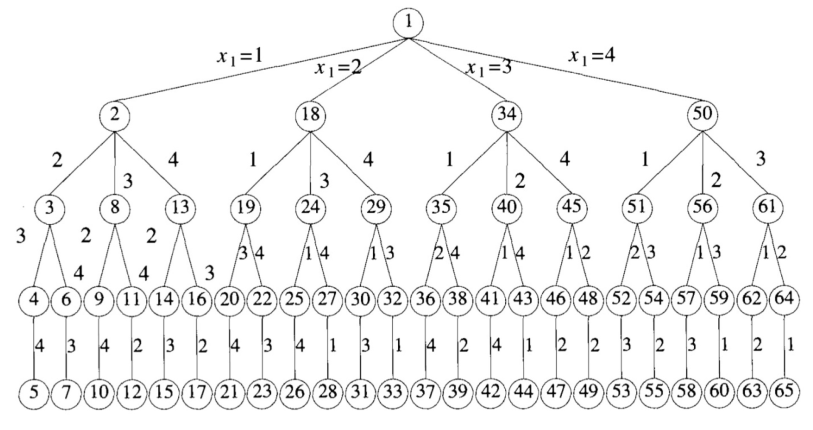
\includegraphics[width=1\textwidth]{./img/C_2.png}
\caption{spazio degli stati 4 regine} \label{FIG:C_2}
\end{figure*}
\textbf{Punto 1}: Presupponiamo di visitare l'albero degli stati tramite le due diverse politiche, effettuando pruning quando necessario.
\begin{itemize}
	\item \textbf{DFS}: La DFS cerca di giungere il prima possibile ad una soluzione, quindi come mostrato in figura~\ref{FIG:C_2_DFS} si scende lungo il ramo più "a sinistra" finchè non si incontra una violazione dei vincoli che induce il pruning (nel nodo 3 ad esempio abbiamo regine in A4 e B3, sulla stessa diagonale).
		Il lato negativo è che spesso la visita in profondità si "infila" in cammini che non portano ad una soluzione, come tutto il sottoalbero generato dalla regina in posizione 2 (A4), potrebbe sembrare conveniente visitare più opzioni possibile in modo da eliminare i cammini che non producono soluzioni il prima possibile.
\begin{figure*}[!ht]
\centering
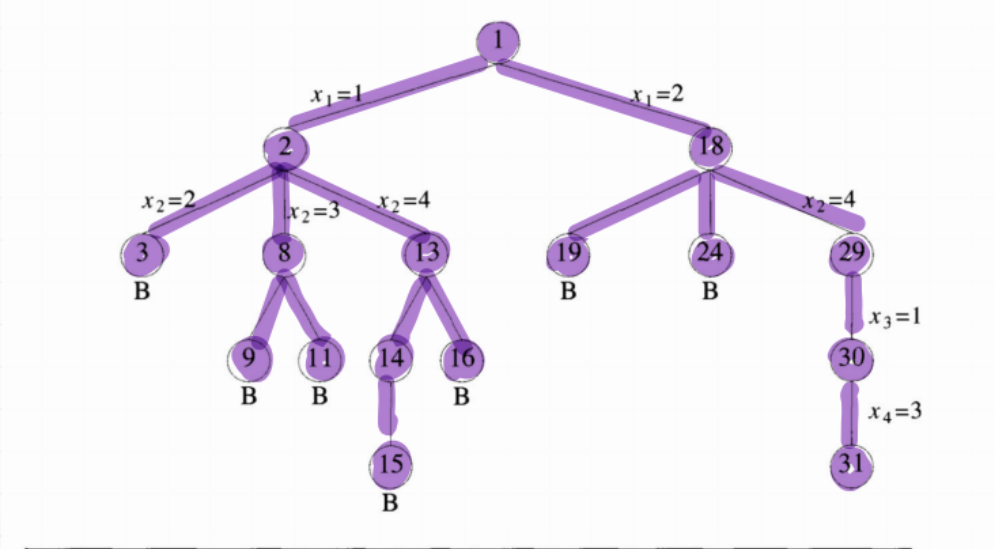
\includegraphics[width=1\textwidth]{./img/C_2_DFS.png}
\caption{Soluzione con DFS} \label{FIG:C_2_DFS}
\end{figure*}\\
	\item \textbf{BFS}:Tramite la visita in ampiezza invece si va ad espandere ogni nodo di un livello dell'albero prima di passare al livello successivo.
		In generale la politica \textit{FIFO} butta via in un sol colpo un sacco di non soluzioni, ma in questo caso prima di incontrare una violazione di qualche vincolo bisogna scendere fino al secondo livello dell'albero, analizzando 16 nodi (che è esattamente il numero di nodi necessari a trovare la \textbf{risposta} con la visita in profondità).
		La politica \textit{LIFO} si dimostra quindi molto meno vantaggiosa, oltretutto si porta dietro un altro svantaggio: se infatti la \textit{FIFO} approfittava dello stack generato dalla ricorsione per mantenere i suoi progressi in memoria nella \textit{LIFO} bisogna costruire una struttura dati atta a mantenere i nodi della "frontiera" in memoria, dato che ogni soluzione viene costruita in parallelo.
		\begin{figure*}[!ht]
\centering
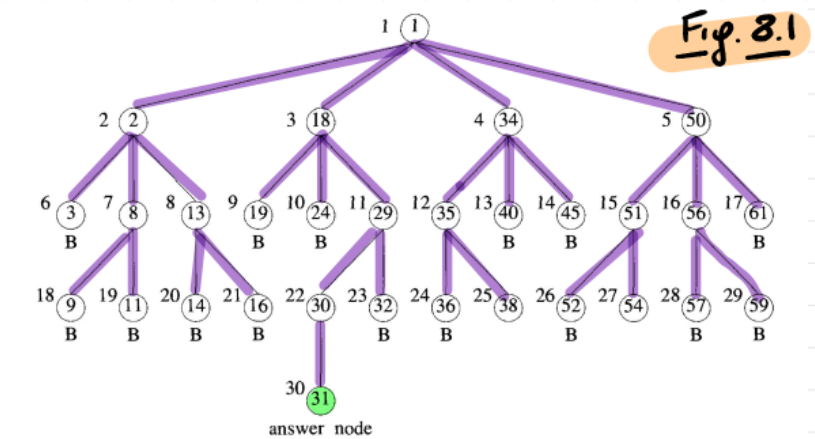
\includegraphics[width=1\textwidth]{./img/C_2_BFS.png}
\caption{Soluzione con BFS} \label{FIG:C_2_BFS}
\end{figure*}
\end{itemize}
\textbf{Punto 2}:
\begin{adjustwidth}{.8cm}{0cm}
	Confrontando le due immagini presenti in figura~\ref{FIG:C_2_DFSvsBFS} notiamo chiaramente che la visita \textit{DFS} è più vantaggiosa in questo caso, giungendo alla soluzione in 16 passi rispetto ai 29 della visita \textit{BFS}.\\
\begin{figure*}[!ht]
\centering
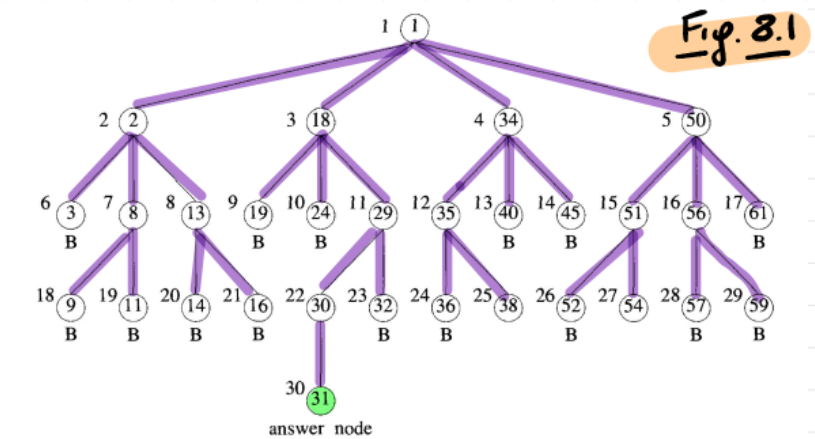
\includegraphics[width=0.49\textwidth]{./img/C_2_BFS.png}
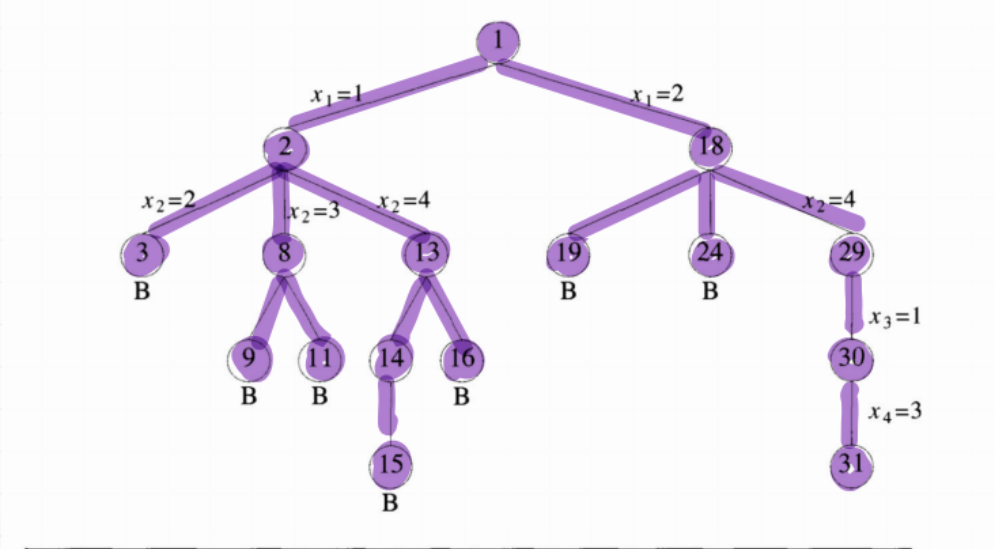
\includegraphics[width=0.49\textwidth]{./img/C_2_DFS.png}
\caption{confronto visita in profondità ed ampiezza} \label{FIG:C_2_DFSvsBFS}
\end{figure*}\\ 
In generale è vero che la politica \textit{FIFO} permette di "buttare via" in un sol colpo un sacco di non soluzioni, ma in questo caso prima di giungere a nodi non accettabili si è obbligati a visitare gran parte dell'albero degli stati.
Sto sì eliminando moltissimi sotto-alberi rispetto alla \textit{DFS} ma per farlo ne sto esplorando molti di più.Più l'albero è ampio rispetto alla sua profondità peggiori sono le prestazioni di una visita in \textit{ampiezza}

%non mi piace proprio questa risposta.


L'ideale sarebbe visitare in ampiezza ma scendere in profondità quando un ramo sembra promettente, per individuare i rami più promettenti si potrebbe ad esempio ordinare i live node minimizzando una delle seguenti proprietà:
\begin{enumerate}
	\item Il numero di nodi nel sottoalbero di $x$ da generare prima di ottenere una \emph{soluzione}.
	\item il numero di livelli che separano il live node dalla risposta.
\end{enumerate}
Il problema derivante dal tentare questo approccio sta proprio nel calcolare le due misure.
Non conoscendo le \textit{soluzioni}, e di conseguenza nemmeno la \textit{risposta}, l'unico modo di effettuare le misure descritte sopra sarebbe quello di esplorare lo spazio degli stati fino ad una \textit{risposta}.
Questa situazione è però paradossale, se conoscessi la risposta non la starei cercando, quindi la misurazione delle due proprietà non è un criterio di ranking applicabile.
\end{adjustwidth}
\subsection{C.3}
\label{SEC:C_3}
\textbf{Punto 1}
\begin{adjustwidth}{.8cm}{0cm}
\begin{definition}
	La \textit{funzione costo} $\hat c(x)$ di un \textit{live node x} è: $$\hat c(x) = f(h(x)) + \hat g(x)$$
\end{definition}
\begin{itemize}
	\item$h$ è una funzione che quantifica il lavoro, quindi $h(x)$ è il lavoro noto svolto fin'ora per arrivare al nodo $x$
	\item$f$ è la funzione \emph{peso} monotona, dato in input il lavoro ottenuto da $h$ fornisce un valore proporzionale ad esso utilizzabile come \emph{peso}
	\item$\hat g$ è una \textit{stima} della funzione non nota $g$.Essendo impraticabile calcolare il valore effettivo $g(x)$, $\hat g(x)$ fornisce una stima di quello che sarà il costo della costruzione di un cammino dal nodo $x$ fino ad una eventuale \textit{risposta} che il sotto-albero di radice $x$ contiene.\\
		la funzione $\hat g$ non è generalizzabile, dipende dal problema.
\end{itemize}
E' necessario introdurre una funzione costo in quanto non è possible calcolare accuratamente il \textit{ranking} di un nodo, bisogna quindi ripiegare su una stima che permetta scegliere in maniera intelligente il prossimo \textit{E-node}.
E' composta principalmente da due parti, il \textit{costo noto} ed il \textit{costo stimato}\\
\begin{figure*}[!ht]
\centering
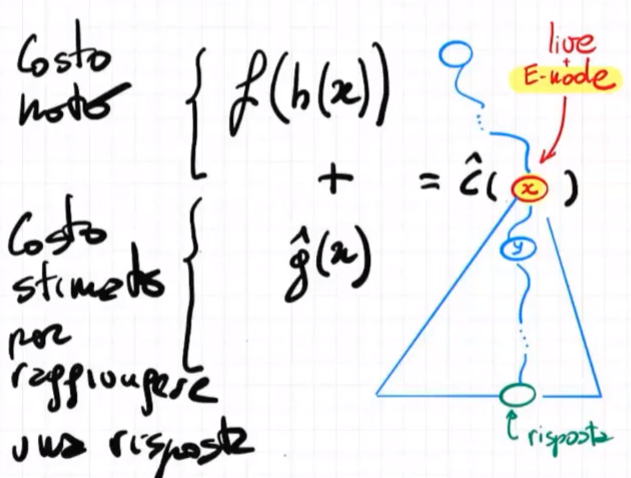
\includegraphics[width=0.4\textwidth]{./img/C_3_punto1.png}
\caption{funzione costo} \label{FIG:C_3_punto1}
\end{figure*}\\
Notiamo anche che dati due nodi $x,y$ se $y$ è un discendente di $x$ ci aspettiamo che la funzione $\hat g(x) > \hat g(y)$, altrimenti la funzione costo è mal formata.
\end{adjustwidth}
\textbf{punto 2}
\begin{adjustwidth}{.8cm}{0cm}
DOPO AVER RICORDATO? cioè devo riscrivere la definizione? mi sembra ridondante.\\
Analizziamo la situazione: $f(h(x)) =0$, in questo caso il \textit{costo noto} non ha influenza sul risultato generato da $\hat c(x)$ e la \textit{funzione costo} può essere riscritta come $$\hat c(x) = \hat g(x)$$
Questo ci riporta ad un algoritmo di \textit{Backtracking}, in quanto non vi è "penalità" nell' espandere nodi in profondità nell'albero degli stati.Considerando che dati due nodi $x,y$ se $y$ è un discendente di $x$ allora $\hat g(x) > \hat g(y)$ la scelta che minimizza la \textit{funzione costo} è sempre quella che espande un nodo di livello successivo, quindi una \textit{D-search}.
Immaginiamo ad esempio due \textit{live node} $x,z$, l' \textit{E-node} è $x$ e genera due discendenti: $w_1, w_2$.
		\begin{align}
			&0 + \hat g(x) < 0 + \hat g(z) \text{ dato che $x$ è \textit{E-node}} \notag \\
			&0 + \hat g(w_1) \leq 0 + \hat g(w_2) < 0 + \hat g(z) \text{ dato che $\hat g$ è monotona} \notag\\
			&\hat c(w_1) \leq \hat c(w_2) < \hat c(z) \notag
	        \end{align}
		Di conseguenza il prossimo \textit{E-node} sarà scelto tra $w_1$ e $w_2$
\end{adjustwidth}
\textbf{punto 3}
\begin{adjustwidth}{.8cm}{0cm}
DOPO AVER RICORDATO? cioè devo riscrivere la definizione? mi sembra ridondante.\\
Analizziamo la situazione: $f(h(x)) \neq 0$, $\hat c(x) = f(h(x)) + \hat g(x)$.\\
Riprendendo l'idea del punto precendente abbiamo due \textit{live node} $x,z$, l'\textit{E-node} è $x$ e genera discendenti chiamati $w_1,..., w_n$.
\begin{align}        
	f(h(x)) + \hat g(x) &< f(h(x)) + \hat g(z) \notag \\
	c(w_1) = (f(h(x) + &\Delta) + (\hat g(x) - \Delta') \notag \\
	c(w_1) = (f(h(x)) + &\hat g(x)) + (\Delta - \Delta') \notag
	\end{align}
	\begin{equation}
	\begin{cases}
		se \; (\Delta - \Delta') &\leq 0 \text{ proseguiamo lungo il ramo di $w_1$} \notag \\
		se \; (\Delta >> \Delta') &\text{ $w_1$ non è un nodo conveniente} \notag
	\end{cases}
	\end{equation}
In questa situazione i valori di $\hat c(w_1), \hat c(w_2), . . . , \hat c(w_n)$ possono superare quelli relativi a live node inseriti nella lista prima di $w_1, w_2, . . . , w_n$ e, quindi, risultare sconvenienti da seguire rispetto ad altri.
\end{adjustwidth}
\subsection{C.4}
Come già mostrato in sezione~\ref{SEC:C_1}, più precisamente in figura~\ref{FIG:C_1} \textit{FIFO} e \textit{LIFO} sono "i due estremi di un ventaglio di possibili criteri di scelta" ed in quanto tali possono essere ottenuti tramite una precisa formulazione della \textit{funzione costo}.
Infatti analizzando la \textit{funzione costo} $\hat c(x) = f(h(x)) + \hat g(x)$ si nota facilmente quali sono le possibili casistiche che possono portare ad un estremo o all'altro.
\begin{itemize}
	\item $\hat c(x) = f(h(x)) + 0$ In questo caso la \textit{funzione costo} non subisce l'influenza del \textit{costo stimato}.
		La \textit{funzione costo} può essere riscritta come $$\hat c(x) = f(h(x))$$
		Intuitivamente i \textit{nodi} più vicini alla radice avranno un costo inferiore, di conseguenza verranno scelti per primi e si verificherà la classica situazione caratteristica delle \textit{Breadth-search}: tutti i nodi appartenenti ad un livello dell'albero verranno esaminati prima di procedere con l' espansione dei nodi del livello successivo.
Immaginiamo ad esempio due \textit{live node} $x,z$, l' \textit{E-node} è $x$ e genera due discendenti: $w_1, w_2$.
                \begin{align}
                        &f(h(x)) + 0 < f(h(z)) + 0 \text{ dato che $x$ è \textit{E-node}} \notag \\
                        &f(h(w_1)) + 0 = f(h(w_1)) + 0 > f(h(z)) + 0 \\
                        &\hat c(w_1) = c(w_2) > \hat c(z) \notag
                \end{align}
Di conseguenza il prossimo \textit{E-node} sarà sicuramente $z$.\\
L'equazione del punto (1) deriva dal fatto che per giungere a $w_1,w_2$ è stato fatto del lavoro in più, esattamente il lavoro necessario ad espandere $x$

	\item $\hat c(x) = 0 + \hat g(x)$ Questa casistica, già affrontata nella sezione~\ref{SEC:C_3} al \textbf{Punto 2} si riconduce ad una \textit{D-search}.
		Se $f(h(x)) =0$ il \textit{costo noto} non ha influenza sul risultato generato da $\hat c(x)$ e la \textit{funzione costo} può essere riscritta come: $$\hat c(x) = \hat g(x)$$
Questo ci riporta ad un algoritmo di \textit{Backtracking}, in quanto non vi è "penalità" nell' espandere nodi in profondità nell'albero degli stati.
Considerando che dati due nodi $x,y$ se $y$ è un discendente di $x$ allora $\hat g(x) > \hat g(y)$ la scelta che minimizza la \textit{funzione costo} è sempre quella che espande un nodo di livello successivo, quindi una \textit{D-search}.
Immaginiamo ad esempio due \textit{live node} $x,z$, l' \textit{E-node} è $x$ e genera due discendenti: $w_1, w_2$.
                \begin{align}
                        &0 + \hat g(x) < 0 + \hat g(z) \text{ dato che $x$ è \textit{E-node}} \notag \\
                        &0 + \hat g(w_1) \leq 0 + \hat g(w_2) < 0 + \hat g(z) \text{ poichè $\hat g$ è monotona} \notag\\
                        &\hat c(w_1) \leq \hat c(w_2) < \hat c(z) \notag
                \end{align}
Di conseguenza il prossimo \textit{E-node} sarà scelto tra $w_1$ e $w_2$

\end{itemize}
\subsection{C.5}

\subsection{C.6}
L'idea da cui partire per sviluppare una \textit{funzione costo} per \imp{SubsetSum} è quella di individuare un intervallo di valori al cui interno è compreso il valore \emph{s} del problema \imp{SubsetSum} $X =({X_0 ... X_{n-1}},S)$ 
Per chiarezza presentiamo con $X_k$ il valore numerico di un elemento, $x_k \in {0,1}$ indica se il numero è inserito nell'insieme o no.
Come descritto nella sezione~\ref{SEC:C_3} la \textit{funzione costo} $\hat c$ è composta da una \textit{parte nota} ed una \textit{parte stimata}.
$$\hat c(x[0..j)) = f(h(x[0..j))) + \hat g(x[0..j))$$
\begin{itemize}
	\item La parte nota è facilmente individuabile come la somma dei numeri già inseriti nell'insieme.$$ f(h(x[0..j)))=\sum_{0 \leq k < j} X_kx_k$$
	\item La parte stimata viene calcolata in modo che valga la seguente condizione:
		$$ f(h(x[0..j))) + \hat g(x[0..j)) - V \leq S \leq f(h(x[0..j))) + \hat g(x[0..j)) $$
	Rivmuovendo $V$ ottengo una approssimazione per difetto di $S$, se non lo rimuovo ottengo una approssimazione per eccesso.
	Se però $V$ viene preso dall'insieme $X$ diventa l'elemento che se tolto dalla somma degli elementi che mi rimangono da inserire fornisce la migliore approssimazione per difetto/eccesso di $S$
	$ \hat g(x[0..j))=\sum_{j \leq k < split} X_k$ in cui il valore split è t.c:
	$$\sum_{j \leq k < split-1} X_k \leq S \leq \sum_{j \leq k < split} X_k$$
\end{itemize}
Lo scopo di questa funzione costo è esplorare in maniera più intelligente lo spazio delle soluzioni, la strategia \textit{LC} diventa la strategia di scelta del prossimo \textit{E-node} tra tutti i possibili \textit{live-node}.
Ma a parità di \imp{costo} bisogna comunque affidarsi ad uno dei due criteri (\textit{LIFO/FIFO}) ma si potrebbe pensare anche di non affidarsi ad un criterio fisso e decidere randomicamente di volta in volta, per introdurre "perturbazioni" che riducano il rischio di svolgere ripetutamente scelte sbagliate.

E naturalmente anche possibile migliorare l'efficenza di questa visita tramite pruning rimuovendo i rami dell'albero il cui valore $ f(h(x[0..j))) + \hat g(x[0..j)) - V > S$.Non ha infatti senso esplorare i sottoalberi che generano, in quanto non possono contenere soluzioni.
%oltretutto nella funzione costo cerco di minimizzare il lower bound, altrimenti sarebbe un branch and bound
%non mi convince per nulla la cosa di LIFO/FIFO sembra che il prof voglia che analiziamo il suo codice e ne traiamo delle conclusioni.
\subsection{C.7}
Per raffigurare matematicamente la scacchiera si può immaginare un insieme $X$ con $|X| = n*n$, essendo le regine 4 la scacchiera ha 64 caselle e quindi $|X| = 64$ in questa istanza.
\begin{itemize}
	\item La parte nota è data dalle caselle della scacchiera non occupabili, quindi le celle in cui è presente una regina o in cui una regina può muoversi e di conseguenza mangiare
\end{itemize}

%DISEGNO SCACCHIERA + ALBERO?

\subsection{C.8}
La qualità di tutti gli algoritmi greedy può essere migliorata ordinando gli elementi in base al rapporto $\frac{valore}{peso}$, operazione con costo $O(n\log_n)$.
In generale le approssimazioni fornite da algoritmi greedy per la risoluzione di \imp{Knapspack} sono molto vicine alla risposta. %il prof se non sbaglio diceva 80%
Per entrambi gli algoritmi presupponiamo tre strutture dati di dimensione $n$, "vettore" $w$ dei pesi, "vettore" $p$ dei profitti e "vettore" $x$ delle scelte. $x[j] \in {0,1}$ indica se l'elemento di indice $j$ è inserito o no nello zaino.
%mi fa schifo il temine vettore, vorrei indicare una generica struttura dati.
\begin{itemize}
	\item \textbf{Greedy}: 
		\begin{lstlisting}[language=Matlab]
	w_tot = 0
	z = 0
	for j = 0 to n do
		if w_tot + w[j] <= c then
			x[j] = 1
			w_tot = w_tot + w[j]
			z = z + p[j]
		else x[j] = 0
		\end{lstlisting}
		L'algoritmo può essere intuitivamente riassunto in 3 passi
		\begin{enumerate}
			\item prova ad inserire un elemento di peso $w[j]$ nello zaino
			\item se l' aggiunta dell' elemento non causa il superamento del limite $c$ inseriscilo, passa al prossimo altrimenti.
			\item analizzati tutti gli elementi concludi.
		\end{enumerate}
	\item \textbf{Greedy-split}:
		\begin{lstlisting}[language=Matlab]
	w_tot = 0
	z = 0
	j = 0
	while w_tot + w[j] <= c
			x[j] = 1
			w_tot = w_tot + w[j]
			z = z + p[j]
			j = j + 1
		\end{lstlisting}
		Questo algoritmo è ancora meno preciso dell' algoritmo \textbf{greedy}, in quanto interrompe la ricerca appena si incontra un elemento che causa il superamento del limite $c$.
		E' però anche più efficiente, non dovendo analizzare altri elementi che rischiano di non poter essere inseriti nello zaino.
		\begin{enumerate}
			\item prova ad inserire un elemento di peso $w[j]$ nello zaino
			\item se l' aggiunta dell' elemento non causa il superamento del limite $c$ inseriscilo, altrimenti concludi la visita.
		\end{enumerate}
\end{itemize}
Entrambi gli algoritmi soffrono di un problema, sono \textit{potenzialmente pessimi}, ma non è questo il caso presentato nella domanda.
$$(\vec w = (1,M)), \vec p = (3,M), 2M$$
Questo caso ha un particolarità, analizzando i pesi si può notare che $p_{max} = M +1$ essendoci solo due elementi, uno di peso $M$ l'altro di peso $1$.La particolarità è che $2M > M + 1 \forall M > 0$, quindi se lo zaino ha una capienza maggiore di $0$ potrà sempre contenere tutti gli elementi che siamo intenzionati ad inserire.
\begin{figure*}[!ht]
\centering
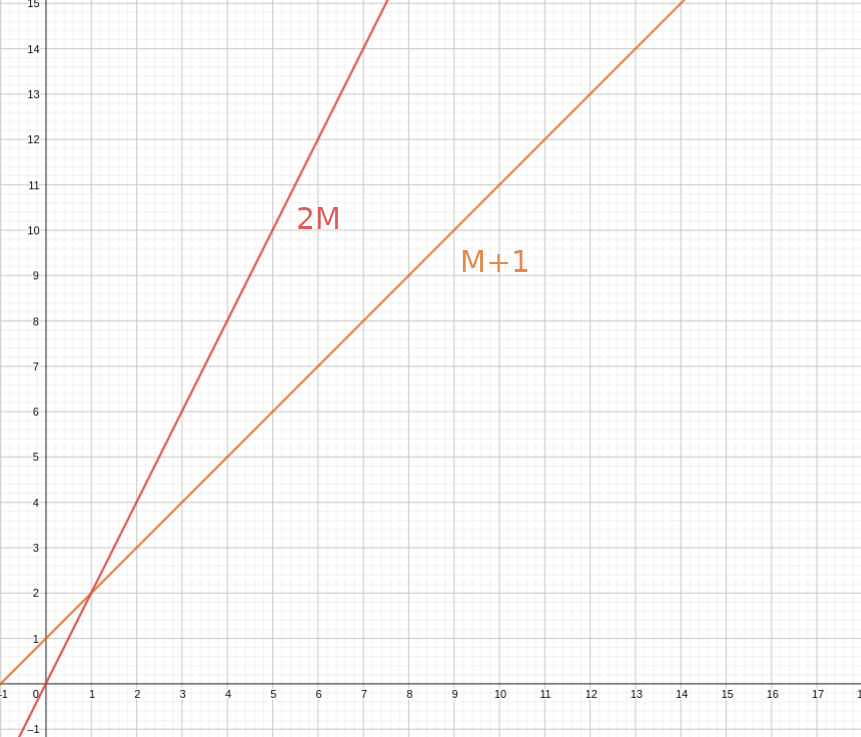
\includegraphics[width=0.5\textwidth]{./img/C_8.png}
\caption{Dimensione soluzione vs spazio al crescere di M} \label{FIG:C_8}
\end{figure*}\\
In questo caso \textbf{Greedy-split} si dimostra perfettamente identico in termini di soluzione a \textbf{Greedy}, in quanto non si incontra mai un elemento che causa il superamento del limite $c$, unica differenza dei due algoritmi.
\subsection{C.9}
La qualità di tutti gli algoritmi greedy può essere migliorata ordinando gli elementi in base al rapporto $\frac{valore}{peso}$, operazione con costo $O(n\log_n)$.
In generale le approssimazioni fornite da algoritmi greedy per la risoluzione di \imp{Knapspack} sono molto vicine alla risposta. %il prof se non sbaglio diceva 80%
Per entrambi gli algoritmi presupponiamo tre strutture dati di dimensione $n$, "vettore" $w$ dei pesi, "vettore" $p$ dei profitti e "vettore" $x$ delle scelte. $x[j] \in {0,1}$ indica se l'elemento di indice $j$ è inserito o no nello zaino.
%mi fa schifo il temine vettore, vorrei indicare una generica struttura dati.
Inoltre supponiamo non esista alcun elemento di indice $j$ tale che $p[j] > c$.
\begin{itemize}
\item \textbf{Greedy-split}:
		\begin{lstlisting}[language=Matlab]
	w_tot = 0
	z = 0
	j = 0
	while w_tot + w[j] <= c
			x[j] = 1
			w_tot = w_tot + w[j]
			z = z + p[j]
			j = j + 1
		\end{lstlisting}
		Questo algoritmo interrompe la ricerca appena si incontra un elemento che causa il superamento del limite $c$.
		\begin{enumerate}
			\item prova ad inserire un elemento di peso $w[j]$ nello zaino
			\item se l' aggiunta dell' elemento non causa il superamento del limite $c$ inseriscilo, altrimenti concludi la visita.
		\end{enumerate}
	Questo algoritmo, come \textbf{Greedy} soffre di un problema, è \textit{potenzialmente pessimo}.\\
	L' istanza di \imp{KP} presentata nella domanda è un esempio di questa situazione:
	$$(\vec w = (1,M), \vec p = (2,M), M)$$
	Infatti ordinando gli elementi per $pw = \frac{profit}{weight}$ notiamo che 
	\begin{align}
		pw_1  &> pw_2 \notag \\
		\frac{2}{1} &> \frac{M}{M} = 1 \notag
	\end{align}
	Seguendo l'algoritmo \textbf{Greedy-split} verrà scelto l'elemento con $pw$ maggiore, cioè l'elemento con indice 1.\\
	Finchè $M \leq p_1$ questo ci fornisce una \textit{risposta} in quanto il scegliendo l'elemento con indice 1 abbiamo un profitto maggiore o uguale di quello che avremmo scegliendo l'elemento con indice 2 (quello con \textit{peso} e \textit{profitto} pari ad $M$.\\
	Quando però $ M > p_1$ l'algoritmo sceglie erroneamente, infatti considerando $M =3$  il profitto ottenuto scegliendo l'elemento di indice 1 è 2, mentre il profitto ottenibile scegliendo il secondo elemento è 3.\\
	Il rapporto $\frac{profitto \; ottenuto}{profitto \; ottimo}$ decresce al crescere di $M$ rendendo sempre più "incorretta" la soluzione offerta da \textbf{Greedy-split}. 
\begin{figure*}[!ht]
\centering
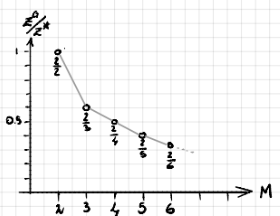
\includegraphics[width=0.5\textwidth]{./img/C_9_greedy.png}
\caption{Qualità della soluzione di \textbf{Ext-Greedy} al crescere di $M$} \label{FIG:C_9_greedy}
\end{figure*}\\
\item \textbf{Ext-Greedy}:
		\begin{lstlisting}[numbers=left,firstnumber=1,language=Matlab, stepnumber=1, xleftmargin=50pt]
w_tot = 0
z=0
for j = 0 to n do
	if w_tot + w[j] <= c then
		x[j] = 1
		w_tot = w_tot + w[j]
		z = z + p[j]
	else x[j] = 0
for j = 0 to n do
	if p[j] > z
		z = p[j]
		for k = 0 to n do x[k] = 0
		x[j] = 1
		\end{lstlisting}
		\begin{enumerate}
			\item prova ad inserire un elemento di peso $w[j]$ nello zaino (riga 4)
			\item se l' aggiunta dell' elemento non causa il superamento del limite $c$ inseriscilo, passa al prossimo altrimenti. (righe 3-8)
			\item analizzati tutti gli elementi concludi il ciclo.
			\item confronta il valore ottenuto dal ciclo con il valore di ogni oggetto, se esiste un elemento che fornisce un risultato migliore di quello trovato nel ciclo (righe 3-8) allora inserisco solo quell'elemento nello zaino. $Z_{risposta} = max\{z, max\{p_1 ... p_n\}\}$
		\end{enumerate}
		Questo algoritmo risolve il problema degli algoritmi \textbf{Greedy} e \textbf{Greedy-split} in qquanto se si verifica una situazione analoga a quella presentata nella domanda $(\vec w = (1,M), \vec p = (2,M), M)$ verrà preso l'elemento avente peso e profitto $M$ in quanto il suo profitto è superiore al profitto offerto dagli elementi inseriti in base all'incremento locale.
\begin{figure*}[!ht]
\centering
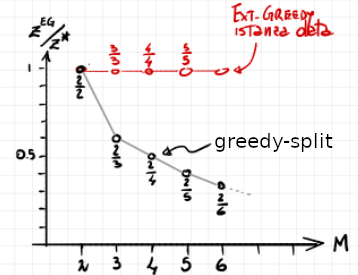
\includegraphics[width=0.5\textwidth]{./img/C_9_ext.png}
\caption{Comportamento \textbf{Ext-Greedy} rispetto a \textbf{Greedy-split}} \label{FIG:C_9_ext}
\end{figure*}\\
\end{itemize}
\subsection{C.10}
\textbf{Ext-Greedy}:
		\begin{lstlisting}[numbers=left,firstnumber=1,language=Matlab, stepnumber=1, xleftmargin=10pt]
w_tot = 0
z=0
for j = 0 to n do
	if w_tot + w[j] <= c then
		x[j] = 1
		w_tot = w_tot + w[j]
		z = z + p[j]
	else x[j] = 0
for j = 0 to n do
	if p[j] > z
		z = p[j]
		for k = 0 to n do x[k] = 0
		x[j] = 1
		\end{lstlisting}
		\begin{enumerate}
			\item prova ad inserire un elemento di peso $w[j]$ nello zaino (riga 4)
			\item se l' aggiunta dell' elemento non causa il superamento del limite $c$ inseriscilo, passa al prossimo altrimenti. (righe 3-8)
			\item analizzati tutti gli elementi concludi il ciclo.
			\item confronta il valore ottenuto dal ciclo con il valore di ogni oggetto, se esiste un elemento che fornisce un risultato migliore di quello trovato nel ciclo (righe 3-8) allora inserisco solo quell'elemento nello zaino. $Z_{risposta} = max\{z, max\{p_1 ... p_n\}\}$
		\end{enumerate}
	
\subsection{C.11}
\subsection{C.12}
\subsection{C.13}
\subsection{C.14}
Nella creazione di un algoritmo \textit{Branch\&Bound} per \emph{KP} la prima cosa da fare è stabilire una \textbf{funzione costo}.Questo può essere fatto basandosi sulla gerarchia dei profitti degli algoritmi greedy vista in precedenza.In particolare il costo ad un \textit{E-node} $x[0..j)$ può essere scritto come:
$$\hat{c}(x[0..j)) = f(h(x[0..j))) + \hat{g}(x[0..j))$$
\begin{itemize}
	\item Nella prima parte dell'equazione abbiamo il \textit{costo noto}, che non è altro che la somma di tutti i profitti dei nodi "inseriti nello zaino" fin'ora ed i loro pesi. 
		\begin{equation}
                	f(h(x[0..j))\begin{cases}
			fh.w(x[0..j))= \sum_{0\leq k < j} x_{k}w_{k}\\
			fh.z(x[0..j))= \sum_{0\leq k < j} x_{k}p_{k}\notag
                \end{cases}
	        \end{equation}
	\item La seconda parte di equazione fornisce una stima per eccesso del profitto ottenibile (\textit{Upper bound}).
		\begin{equation}
			\hat{g}(x[0..j))\begin{cases}
				\hat{g}.w(x[0..j))= (\sum_{j\leq k < split} w_{k})+(c-[fh.w(x[0..j)) + \sum_{j\leq k < split} w_{k}]\\
				\hat{g}.z(x[0..j))= (\sum_{j\leq k < split} p_{k})+(c-[fh.w(x[0..j)) + \frac{\sum_{j\leq k < split} w_{k}]}{W_{split}}P_{split} \notag
                	\end{cases}
	        \end{equation}
	\item Una terza misura utile a scrivere un algoritmo \textit{Branch\&Bound} per il problema Knapspack è una stima per difetto (\textit{Lower Bound}), facilmente ottenibile tramite l'algoritmo greedy (o greedy split).
		\begin{align}
				z^g(x[0..j)) &= \sum_{0\leq k < j} x_{k}p_{k} + \sum_{j\leq k < split} p_{k} + \sum_{split < k < n} x_{k}p_{k} \notag \\
			&se \sum_{0\leq k < j} x_{k}w_{k} + \sum_{j\leq k < split} w_{k} + \sum_{split < k < n} x_{k}w_{k}\notag
		\end{align}
\end{itemize}
Una volta descritte le 3 misure si può impostare un algoritmo per la risoluzione \textit{Branch\&Bound} che rispetti la seguente invariante: In qualsiasi istante della visita $lower \; bound < z^* < upper \; bound$\\
L'idea di base è quindi quella di raffinare tramite le diverse iterazioni i due limiti fino ad ottenere la miglior \emph{soluzione} che sarà la \emph{risposta}.\\
\textit{Passo base}:
\begin{adjustwidth}{.8cm}{0cm}
		Non avendo visitato alcun nodo l' \textit{E-node} è la radice dello spazio degli stati.
		Il \textit{lower bound} è quindi l'algoritmo greedy scelto applicato al problema completo, allo stesso modo l' \textit{upper bound} è il risultato dell'algoritmo di soluzione di \emph{LKP} applicato al problema completo.
		In questo stadio la miglior soluzione (che identifichiamo come $x[0..r)$) è la soluzione trovata tramite l'algoritmo greedy.
\begin{figure*}[!ht]
\centering
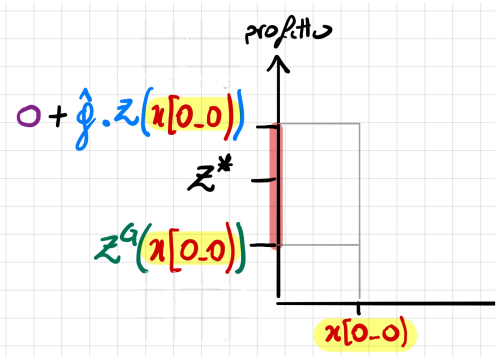
\includegraphics[width=0.7\textwidth]{./img/C14_profitto_z.png}
\caption{Bounds del profitto z} \label{FIG:C14_profitto_z}
\end{figure*}\\
\end{adjustwidth}
\textit{Passo induttivo}:
\begin{adjustwidth}{.8cm}{0cm}
	Al passo induttivo l'attuale \textit{E-node} sarà $x[0..j)$ e il nodo che fornisce la miglior soluzione $x[0..r)$ garantisce un profitto $z^*(x[0..r))$.
	Durante la visita dell' \textit{E-node} si possono presentare 4 situazioni (non esclusive):
	\begin{itemize}
		\item $f(h(x[0..j)) > C$\\
			Non ha senso "espandere" il nodo e proseguire nella visita del sotto-albero $T[0..j)$ in quanto sicuramente non otterremo una risposta avendo superato la capacità massima.Il nodo viene etichettato come \textbf{"completo"}, si sta effettuando \textit{pruning}.
		\item$f(h(x[0..j)) + \hat{g}.z(x[0..j)) < z^*(x[0..r))$\\
			Il profitto ottenibile espandendo il nodo è < dell'approssimazione per difetto trovata in uno dei passi precendenti.Anche inserendo tutti gli oggetti fino a capienza massima non si troverebbe una soluzione migliore di quella attuale (ricordo essere $z^*(x[0..r))$).Il nodo viene etichettato come \textbf{"completo"}, si sta effettuando \textit{pruning}.
\begin{figure*}[!ht]
\centering
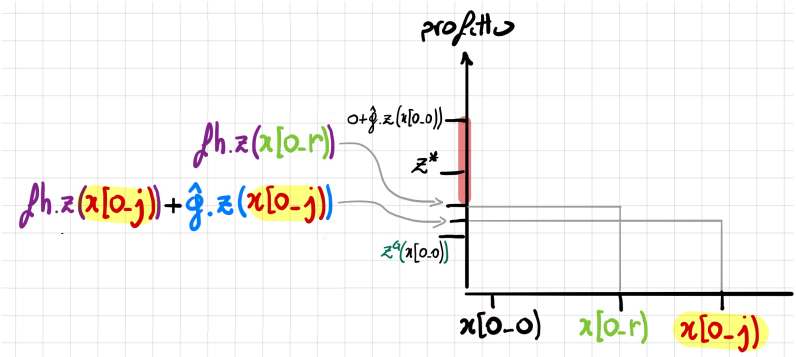
\includegraphics[width=0.7\textwidth]{./img/C14_item2.png}
\caption{nessun miglioramento rispetto alla soluzione del nodo $x[0..r)$} \label{FIG:C14_item2}
\end{figure*}\\
		\item $f(h(x[0..j)) < C \land f(h(x[0..j)) + \hat{g}.z(x[0..j)) > z^*(x[0..r))$\\
			Il sottoalbero $T[0..j)$ può ancora generare \textit{soluzioni}, fra queste potrebbe essere presente la \textit{risposta}.E quindi necessario \textbf{espandere} il nodo e continuare l'esplorazione del sottoalbero.
		\item $f(h(x[0..j)) < C \land f(h(x[0..j)) > z^*(x[0..r))$\\
			E' stata trovata una \textit{soluzione} che migliora il profitto $z^*(x[0..r))$, viene salvata ed i passi successivi faranno riferimento al profitto generato da $x[0..j)$.
	\end{itemize}
	\begin{figure*}[!ht]
\centering
\textbf{$((2,4,6,9),(10,10,12,18),15) \in KP$}
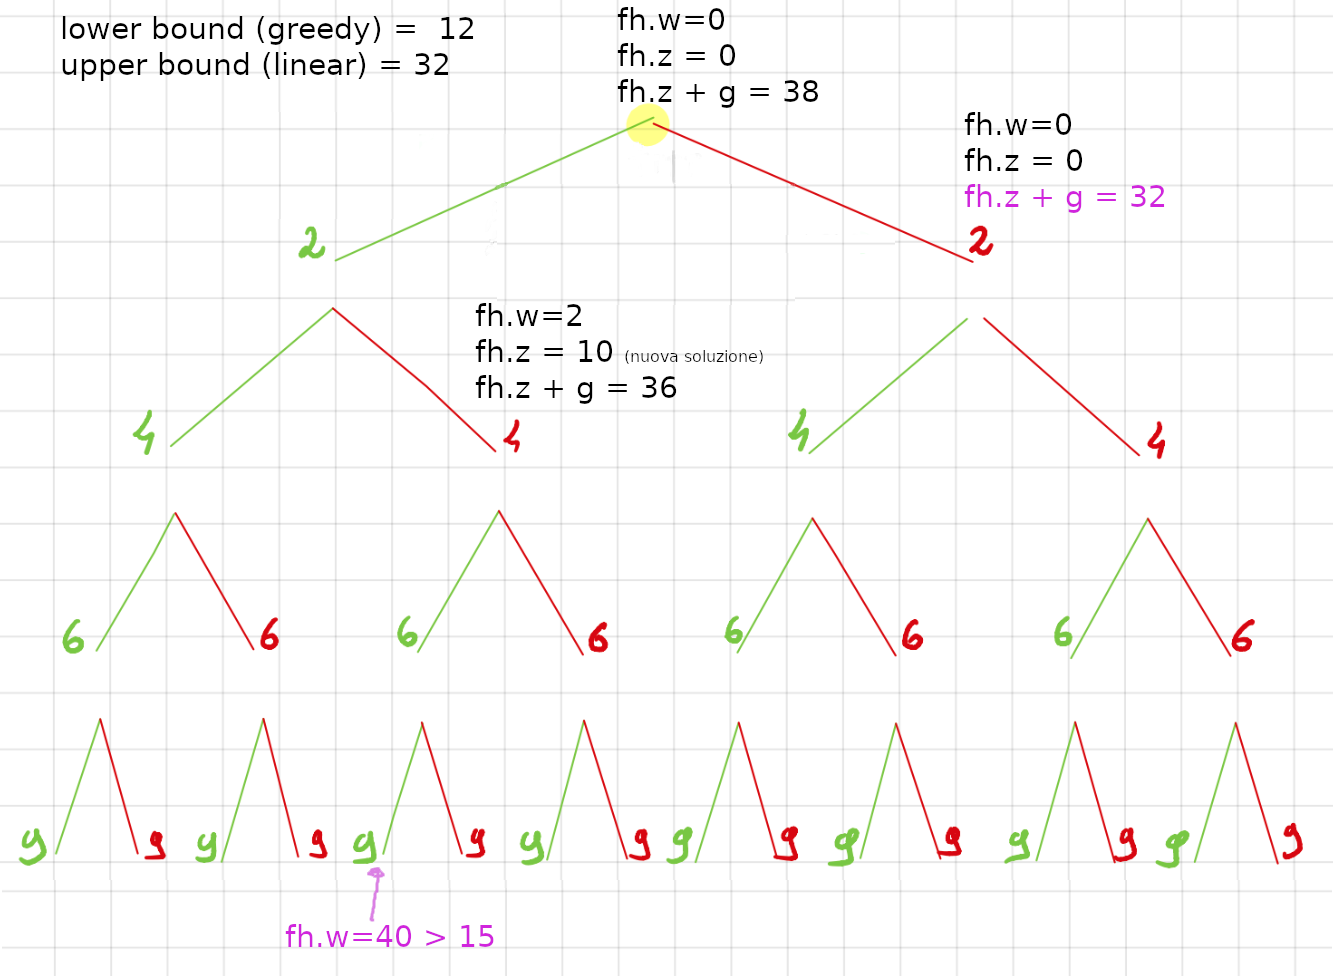
\includegraphics[width=1\textwidth]{./img/C14_BB_manuale.png}
\caption{Esempio di Branch\&Bound} \label{FIG:C14_BB_manuale}
\end{figure*}
	La cosa non specificata dall'algoritmo è il criterio di scelta del prossimo \textit{E-node} tra i vari \textit{live-nodes} disponibili.Utilizzando un criterio FIFO si ottengono buoni risultati, ma usando una tecnica \emph{least-cost} si è scoperto sperimentalmente che le prestazioni sono migliori.
	Intuitivamente ci sono due motivi per questo: in primis se $z^{LP} = Z^*$ è possibile che venga trovata una soluzione che sappiamo con certezza essere anche \textit{risposta}, si può quindi fare pruning dei restanti rami.
	In secondo luogo è possibile che giungendo "prima" alle \textit{soluzioni} migliori il valore di $z^*(x[0..r))$ cresca rapidamente causando il "rifiuto" di nodi che con una politica FIFO sarebbero stati espansi.(I nodi vengono rifiutati per la situazione 2)
\end{adjustwidth}
\section{Problemi computazionali}
\subsection{D.2}
Dimostrare che i problemi \emph{KP} e \emph{Bounded-KP} sono equivalenti.\\Cioè $KP \Leftrightarrow BKP$.\\
\begin{dimostrazione}
	$KP \Rightarrow BKP$: ogni problema \emph{KP} è un problema \emph{BKP}.\\
	La dimostrazione è immediata in quanto un generico problema\\$((P_1, ... ,P_n),(W_1, ... ,W_n),C)\in KP$ può essere riscritto come\\ $((P_1, ... ,P_n),(W_1, ... ,W_n),(1, ... ,1),C) \in BKP$.

	$KP \Leftarrow BKP$: ogni problema \emph{BKP} è un problema \emph{KP}.\\
	per prima cosa introduciamo $B_i + 1$ nuove variabili, $\forall i \in B_1 ... B_n$.\\
	Avremo quindi
	\begin{align}
		x_{0}', ... ,&x_{b_i}' \in \{0,1\}  \notag \\
   		&\;\;\vdots \notag \\
		x_{0}^n, ... ,&x_{b_i}^n \in \{0,1\}  \notag 
	\end{align}
	Queste variabili indicano "quanti" oggetti di tipo $x^i$ sto prendendo, quindi 
	\begin{equation}
		x_{j}^i=\begin{cases}
      		0\; se\; x_i = 0\\
      		1\; se\; x_i = j \notag
    		\end{cases}
	\end{equation}
	Il problema è diventato un esempio di \emph{BKP} di questo tipo:
	\begin{center}
		\scalebox{0.89}{$((p_1, 2p_1 ,...,b_1p_1, ... ,p_n, 2p_n, ..., b_np_n),(w_1, 2w_1 ,...,b_1p_1, ... ,w_n, 2w_n, ..., b_nw_n),C))$}\\
		$maximize \; \sum_{i=1}^{n} \sum_{j=0}^{b_i} p_j*j*x^i_j$\\
		$subject \; to \; \sum_{i=1}^{n} \sum_{j=0}^{b_i} w_j*j*x^i_j$\\
		con la condizione aggiuntiva $ \forall i \sum_{j=0}^{b_i} x_j^i = 1$
	\end{center}
	In modo che  si possano prendere solo $j$ oggetti fi tipo $x^i$
	%non posso prendere 5 x', e poi 3 x', sarebbe come prendere 8 x'
	DA FINIRE CON OSSERVAZIONE DEL PROF RIGUARDO AL FATTO DI DOVER DIMOSTRARE LA RISOLVIBILITà
\end{dimostrazione}
\end{document}
